\documentclass[conference]{IEEEtran}
\IEEEoverridecommandlockouts
\usepackage{cite}
\usepackage{amsmath,amssymb,amsfonts}
\usepackage{graphicx}
\usepackage{booktabs}
\usepackage{algorithm}
\usepackage[noend]{algpseudocode}
\usepackage{microtype}
\usepackage{url}
\usepackage{balance}
\newcommand{\NTotal}{960}
\newcommand{\NTest}{770}
\newcommand{\NCal}{190}
\newcommand{\NDet}{595}
\newcommand{\NNonDet}{175}
\newcommand{\NNuis}{345}
\newcommand{\NLegitDet}{263}
\newcommand{\NCellDet}{616}
\newcommand{\NNuisDeg}{21}
\newcommand{\NLegitNuisDeg}{6}
\newcommand{\ThetaLocal}{0.70}
\newcommand{\GammaLocal}{0.06}
\newcommand{\ThetaGlobal}{0.50}
\newcommand{\GammaGlobal}{0.70}
\newcommand{\AlgAcc}{89.9}
\newcommand{\AlgAccLo}{87.4}
\newcommand{\AlgAccHi}{92.3}
\newcommand{\AlgAAR}{96.6}
\newcommand{\AlgUAR}{1.8}
\newcommand{\AlgUBR}{1.7}
\newcommand{\AlgMis}{2.5}
\newcommand{\AlgFA}{10.3}
\newcommand{\BayAcc}{73.8}
\newcommand{\BayMis}{0.0}
\newcommand{\BayFA}{0.0}
\newcommand{\BayAAR}{82.3}
\newcommand{\GloAcc}{82.0}
\newcommand{\BoneAcc}{46.6}
\newcommand{\BoneMis}{47.5}
\newcommand{\BoneFA}{19.0}
\newcommand{\BthreeAcc}{69.2}
\newcommand{\BthreeUBR}{56.0}
\newcommand{\BthreeFA}{36.5}
\newcommand{\McBoneRef}{285}
\newcommand{\McBoneOther}{27}
\newcommand{\McBthreeRef}{155}
\newcommand{\McBthreeOther}{32}
\newcommand{\FwdGlo}{27.0}
\newcommand{\FwdAlg}{85.4}
\newcommand{\FwdBayLegit}{83}
\newcommand{\FwdNDet}{89}
\newcommand{\NoNuisAcc}{98.4}
\newcommand{\NuisAcc}{80.5}
\newcommand{\FATotal}{27}
\newcommand{\FAMisread}{19}
\newcommand{\FAGlare}{9}
\newcommand{\FABoth}{3}
\newcommand{\FANeither}{2}
\newcommand{\MassBig}{96.2}
\newcommand{\MassSmall}{86.7}
\newcommand{\MassZero}{91.8}
\newcommand{\Cloned}{70.0}
\newcommand{\FAlgAcc}{84.2}
\newcommand{\FAlgUAR}{8.9}
\newcommand{\FAlgMis}{1.0}
\newcommand{\FGloAcc}{74.8}
\newcommand{\FBayAcc}{68.1}
\newcommand{\FBthreeAcc}{60.7}
\newcommand{\AbFullAAR}{96.6}
\newcommand{\AbNoQAAR}{42.9}
\newcommand{\AbNoQUBR}{53.1}
\newcommand{\AbNoQFA}{30.8}
\newcommand{\AbNoVisDrop}{13.3}
\newcommand{\AbNoVisFA}{3.4}
\newcommand{\AbFwdFull}{85.4}
\newcommand{\AbFwdNoVis}{27.0}
\newcommand{\AbNoSealAcc}{0.901}
\newcommand{\AbNoSealFA}{5.7}
\newcommand{\AbDoorFull}{98.9}
\newcommand{\AbDoorNoSeal}{85.1}
\newcommand{\SwNuisZeroAcc}{100.0}
\newcommand{\SwNuisFourAcc}{73.3}
\newcommand{\SwNuisFourUAR}{11.6}
\newcommand{\SwNuisMaxMis}{3.2}
\newcommand{\SwSigFourBthreeFA}{81.7}
\newcommand{\SwSigFourBoneMis}{66.7}
\newcommand{\SwSigFourAlgAcc}{81.1}
\newcommand{\SwSigFourAlgUAR}{9.7}
\newcommand{\SwPoseMinAlg}{91.4}
\newcommand{\SwPoseMaxAlg}{94.5}
\newcommand{\VisGloPose}{0.409}
\newcommand{\VisGloNoPose}{0.015}
\newcommand{\VisGloMark}{0.031}
\newcommand{\VisLocIntactMax}{0.009}
\newcommand{\VisLocMarkMin}{0.089}

\newcommand{\LEG}{\textsc{leg}}
\newcommand{\DEG}{\textsc{deg}}
\newcommand{\IND}{\textsc{ind}}
\newcommand{\ANOM}{\textsc{anom}}
\newcommand{\INTACT}{\textsc{intact}}
\newcommand{\UNK}{\textsc{unk}}

\makeatletter
\newcommand{\linebreakand}{\end{@IEEEauthorhalign}\hfill\mbox{}\par\vspace{-10pt}\mbox{}\hfill\begin{@IEEEauthorhalign}}
\makeatother
\begin{document}

\title{TriNetra-Link: Quality-Aware Custody-Stage Attribution with Selective Abstention for E-Commerce Parcel Disputes}

\author{
\IEEEauthorblockN{Sanjai L}
\IEEEauthorblockA{\textit{Dept. of AI \& Data Science}\\
\textit{Saveetha Engineering College}\\
Chennai, India\\
sanjaioff@gmail.com}
\and
\IEEEauthorblockN{Dharshan D}
\IEEEauthorblockA{\textit{Dept. of AI \& Data Science}\\
\textit{Saveetha Engineering College}\\
Chennai, India\\
dharshandhiren@gmail.com}
\and
\IEEEauthorblockN{Kanagavel A. K.}
\IEEEauthorblockA{\textit{Dept. of AI \& Data Science}\\
\textit{Saveetha Engineering College}\\
Chennai, India\\
kanagavel@gmail.com}
\linebreakand
\IEEEauthorblockN{Dr. S. Shanmuga Priya}
\IEEEauthorblockA{\textit{Dept. of Artificial Intelligence}\\
\textit{Saveetha Engineering College}\\
Chennai, India\\
shanmugapriyas@saveetha.ac.in}
\and
\IEEEauthorblockN{Dr. Lavanya G}
\IEEEauthorblockA{\textit{Dept. of Artificial Intelligence}\\
\textit{Saveetha Engineering College}\\
Chennai, India\\
lavanya@saveetha.ac.in}
}

\maketitle

\begin{abstract}
When a returned parcel arrives lighter than it left or under a different seal, the return hub sees only the final state, and current practice tends to charge the customer. TriNetra-Link records weight, seals, identifiers and photographs at four checkpoints and assigns such a discrepancy to forward transit, customer custody or reverse transit. A quality gate first scores every checkpoint from metadata alone; weights, seals, identifiers and registered photographs are then compared with the origin checkpoint. A stage is named only when the checkpoints on both sides of it are trusted; otherwise TriNetra-Link abstains and reports whether the evidence was degraded or the stage indistinguishable. All accuracy figures in this paper come from simulation. The \NTotal-journey benchmark draws scale faults, poor photographs, unreported glare and misread identifiers independently of the staged scenario. On its \NTest{} test journeys the interval rule assigned \AlgAcc\% of determinable journeys to the correct stage and abstained on \AlgAAR\% of the others. It blamed the customer wrongly in \AlgMis\% of cases; inspection at the return hub alone did so in \BoneMis\%. A global structural-similarity score reacted more to camera pose than to tampering, and a registered, glare-masked local comparison raised accuracy from \GloAcc\% to \AlgAcc\%. Two real parcels served only as a feasibility check; on one of them a framing difference alone triggered the visual test, which the capture application now guards against.
\end{abstract}

\begin{IEEEkeywords}
chain of custody, stage attribution, selective prediction, evidence quality, reverse logistics, simulation
\end{IEEEkeywords}

\section{Introduction}
In 2024 India's National Consumer Helpline registered 440,185 e-commerce grievances, more than for any other sector~\cite{nch1951}. Of the 397,333 recorded up to 30~November 2024, 54,563 concerned a wrong product, 53,285 a defective or damaged product and 15,077 a missing product or accessory, together 30.9\% of the total~\cite{nch2442}. These are complaints, not proven tampering, but they show how often a parcel's physical state is disputed.

A discrepancy found at the return hub may have arisen in forward transit, in customer custody or in reverse transit, and each possibility points to a different party. Because the hub can inspect only what arrives, the cost tends to fall on the customer. Recording evidence at every handover helps only if the evidence is usable. Field photographs are often dark or blurred, scales report errors, identifiers are misread and glare covers seals. A rule that blames the stage before the first detected change shifts blame downstream whenever an earlier checkpoint recorded nothing usable, so an attribution method must recognise insufficient evidence and say so.

The paper makes four contributions. We formulate custody-stage attribution with two distinct abstentions, for degraded and for indistinguishable evidence (Section~\ref{sec:problem}). We describe TriNetra-Link: a metadata-only quality gate, a reference-trust rule, three reconcilers, a deterministic interval rule and a quality-weighted Bayesian variant (Section~\ref{sec:method}). We build a simulation benchmark whose nuisance effects are independent of the staged scenario, with baselines, ablations and sweeps (Sections~\ref{sec:sim}--\ref{sec:results}). Finally, we give evidence that global structural similarity tracks camera pose more than tampering, that a registered local comparison corrects this, and, from two real captures, that photograph framing is the next problem. Section~\ref{sec:disc} covers limitations.

\section{Related Work}
\emph{Returns and disputes.} Studies of returns model customers: Shang et~al.~\cite{shang} derive refund policies for worn-and-returned items and Karl~\cite{karl} reviews return forecasting. Dispute tools work on records: Shih et~al.~\cite{shih} store return steps in Ethereum smart contracts, Tsurel et~al.~\cite{tsurel} predict marketplace dispute outcomes from case text, and GS1 EPCIS~2.0~\cite{epcis} standardises the exchange of supply-chain events with sensor data. EPCIS could carry our checkpoint records, but none of these works judges a physical discrepancy or the evidence behind it.

\emph{Parcel inspection.} Elia et~al.~\cite{elia} classify anomalies in returned goods at one warehouse, and TAMPAR~\cite{tampar} compares normalised parcel views with a reference image to detect tampering (81\% accuracy on real images). TAMPAR is closest to our visual reconciler but judges one image pair, without placing the change between handovers or declining on poor photographs.

\emph{Selective prediction.} The reject option goes back to Chow's error--reject trade-off~\cite{chow}; El-Yaniv and Wiener~\cite{elyaniv} formalised risk--coverage and Geifman et~al.~\cite{geifman17,geifman19} carried it to deep networks. There abstention follows model confidence; our gate decides earlier, from the evidence itself (exposure, sharpness, scale status), and each abstention names its reason.

\section{Problem Formulation}\label{sec:problem}
A journey is one parcel observed at $K=4$ checkpoints (Fig.~\ref{fig:pipeline}a): CP1, intake at the origin hub; CP2, the carrier facility; CP3, the doorstep hand-over and later return collection; and CP4, the return hub. Stage $S_k$ is the custody interval between CP$k$ and CP$(k{+}1)$, so $S_1$ is forward transit, $S_2$ customer custody and $S_3$ reverse transit. At each checkpoint an operator records $o_k$: three weighings with scale status, layered seal identifiers and states, serial and IMEI, hashed photographs of named faces, a timestamp, a glare flag and any logged packaging change.

From $o_1,\dots,o_4$ TriNetra-Link returns a label in $\{\LEG, S_1, S_2, S_3, \DEG, \IND\}$: legitimate, a stage, or an abstention because the evidence is degraded (\DEG) or the stage indistinguishable (\IND). The staging log fixes the determinability $\Omega^* \in \{\mathrm{DET}, \DEG, \IND\}$ (Section~\ref{sec:truth}); the aim is to label determinable journeys correctly and abstain on others.

\begin{figure}[t]
\centering
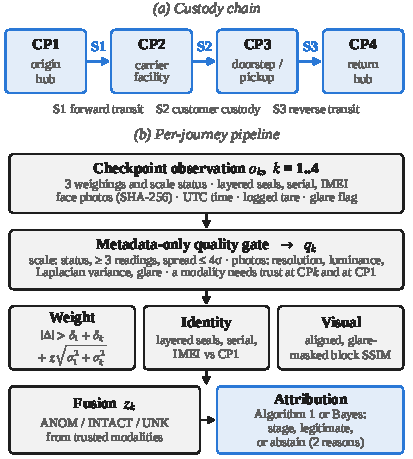
\includegraphics[width=0.78\columnwidth]{fig/fig1_pipeline.pdf}
\caption{TriNetra-Link. (a) Four custody checkpoints and the three stages between them. (b) Per-journey pipeline from checkpoint records to a stage, a legitimate label or a reasoned abstention.}
\label{fig:pipeline}
\end{figure}

\section{Method}\label{sec:method}
\subsection{Metadata-Only Quality Gate}
The gate scores each checkpoint before checkpoints are compared, so a quality score carries no information about the discrepancy. The weight modality scores zero for a scale status other than OK, MANUAL or SETTLED or for fewer than three readings; otherwise the spread $s$ of the readings is compared with the scale's noise standard deviation $\sigma$:
\begin{equation}
q_w = \begin{cases} 1, & s \le 4\sigma\\ \max\!\left(0,\, 1 - \frac{s-4\sigma}{4\sigma}\right), & \text{otherwise.}\end{cases}
\end{equation}
Each photograph is scored on resolution (640$\times$480 floor), mean luminance within [30,\,240], sharpness and glare. Sharpness is the variance of the discrete Laplacian~\cite{pech}, normalised by 2500 with a floor of 0.10, and glare is the fraction of pixels with HSV value above 240 and saturation below 30, with a ceiling of 0.15. The photographic score is the geometric mean over faces, capped at 0.20 when the operator reports glare. Seal and identity evidence is trusted only if the photographs are trusted or the identifiers were scanned or typed. As every comparison is made against CP1, a modality is trusted at CP$k$ only if its score reaches the threshold $\theta$ there and at CP1; a blurred reference photograph cannot anchor a comparison. The checkpoint quality $q_k$ is the largest trusted modality score, and $q_k=0$ when neither photographs nor weights are trusted.

\subsection{Per-Modality Reconciliation}
\emph{Weight.} Let $\tilde w_k$ be the median of the three readings at CP$k$ and $T_k$ the net change in packaging mass logged at permitted packaging changes between CP1 and CP$k$ ($T_k=0$ if the packaging was never changed). A weight anomaly is declared when
\begin{equation}
\left|\tilde w_k - \tilde w_1 - T_k\right| > \delta_1 + \delta_k + z\sqrt{\sigma_1^2+\sigma_k^2},
\end{equation}
where $\sigma_j$ is the single-reading noise standard deviation of the scale used at CP$j$ and $\delta_j$ bounds its linearity drift (largest offset from a reference mass), all in grams. Noise in separate weighings is independent and adds in quadrature~\cite{gum}; drift is systematic and may keep its sign, so the bounds add linearly. We use $z=3$.

\emph{Identity.} A serial or IMEI that differs from CP1 is an anomaly, as is a layered seal that is torn, missing or carries another identifier. An unreadable seal counts as unknown, never intact, and a carrier-replaced flyer is accepted when its new seal is logged.

\emph{Appearance.} The preregistered \emph{global} score rectifies both images of a face to 256$\times$256 pixels with a four-point homography~\cite{hartley} and computes $c^{g}=1-\mathrm{SSIM}$~\cite{ssim}. This score is dominated by small pose differences (Section~\ref{sec:visual}), so we add a \emph{local} score. The CP$k$ image is aligned to the CP1 image by enhanced-correlation-coefficient maximisation~\cite{ecc} under a homography model, with ORB features~\cite{orb} and RANSAC as a second candidate; the alignment with the higher normalised correlation is kept. Regions where glare appears in only one capture are masked; after brightness normalisation and light smoothing, the SSIM map is averaged over $24\times 24$-pixel blocks $b$:
\begin{equation}
c^{l} = \max_b \; \frac{1}{|b|}\sum_{p\in b} \left(1-\mathrm{SSIM}_p\right),
\end{equation}
where $\mathrm{SSIM}_p$ is the SSIM at pixel $p$ and $|b|$ the pixel count of block $b$. A cut tape or re-taped patch then dominates the score instead of being averaged away, and a face is anomalous when its score exceeds $\gamma$. The fused state $z_k$ is \ANOM{} if any trusted modality reports a change, \INTACT{} if none does and at least one matches CP1, and \UNK{} otherwise, with $z_1=\INTACT$.

\subsection{Attribution Rules}
The interval rule (Algorithm~\ref{alg:interval}) returns $S_a$ only when the first trusted anomalous checkpoint $b$ directly follows the last trusted intact one $a$ ($b=a+1$). An untrusted checkpoint between them yields \DEG, and without a trusted CP1 the rule abstains. A checkpoint enters $T$ only through a trusted weight or photograph, each reporting a change or a match, so no trusted checkpoint is \UNK: $a$ always exists, \LEG{} requires every trusted checkpoint to be \INTACT, and line~8 is never reached. A journey with glare reported at two or more checkpoints and no trusted weight or seal anomaly is labelled \IND{} before the rule runs, because only its photographs could have shown the change.

\begin{algorithm}[t]
\caption{Interval attribution}
\label{alg:interval}
\begin{algorithmic}[1]
\Require $q_k$, $z_k$ for $k=1,\dots,K$, with $z_1=\INTACT$ and $z_k\neq\UNK$ if $q_k\ge\theta$; threshold $\theta$
\State $T \gets \{k : q_k \ge \theta\}$
\If{$1 \notin T$} \Return \DEG \EndIf
\State $A \gets \{k \in T : z_k = \ANOM\}$
\If{$A = \emptyset$} \Return \LEG{} if $K \in T$ else \DEG \EndIf
\State $b \gets \min A$; \; $a \gets \max\{k \in T : k < b,\ z_k = \INTACT\}$
\If{$\exists\, k \in (a,b)$ with $q_k < \theta$} \Return \DEG \EndIf
\If{$b = a+1$} \Return $S_a$ \EndIf
\State \Return \IND
\end{algorithmic}
\end{algorithm}

The Bayesian variant scores the hypotheses $h \in \{\LEG, S_1, S_2, S_3\}$, each predicting \INTACT{} before its stage and \ANOM{} after it:
\begin{equation}
P(h \mid o) \propto \pi(h) \prod_k \prod_m p\!\left(o_{k,m} \mid z_k(h)\right)^{q_{k,m}},
\end{equation}
with a uniform prior $\pi(h)$, the quality score $q_{k,m}$ of modality $m$ at CP$k$ as exponent, a true-positive rate of 0.95 and a false-positive rate of 0.05. An untrusted observation contributes a factor of one. The product assumes conditional independence given $h$; correlated readings or photographs can make the posterior overconfident. The variant returns the most probable hypothesis when its posterior is at least $\tau=0.80$ and its bounding checkpoints are trusted, and abstains otherwise.

\section{Simulation Study}\label{sec:sim}
\subsection{Design Rules}
A simulator written by the authors of TriNetra-Link could favour it, so three rules were fixed before any comparison was run. Nuisance effects are drawn independently of the staged scenario, with the same probabilities for every journey. Tamper strength is drawn from wide distributions that reach below every detection limit: weight-matched substitutions, losses of a few grams, cloned seals that reproduce the original identifiers and faint marks. Finally, a fault in a single modality never changes the ground truth.

\subsection{Generative Model}
Each journey draws an item of 55--810\,g plus 75\,g of packaging. At each checkpoint one of three scales is used (noise $\sigma$ of 0.5, 1.0 or 2.0\,g; drift $\delta$ of 0.1, 0.2 or 0.5\,g). Three readings are drawn around the true mass plus a bias within the drift, and packaging moisture varies by 0.6\,g (SD). Three textured faces are photographed with a random corner displacement (8\,px standard deviation at 640$\times$480), exposure gain $1\pm0.08$, sensor noise and JPEG compression. Tampering removes 0\,g with probability 0.25, 2--15\,g with probability 0.25 and 15--200\,g otherwise, never more than 90\% of the item. Seals are torn, replaced, cloned or left unreadable with probabilities 0.35, 0.35, 0.15 and 0.15, the serial changes with probability 0.5, and a mark of random visibility is drawn on the top and seal faces. Table~\ref{tab:nuisance} lists the nuisance effects, each drawn independently per checkpoint.

\begin{table}[t]
\caption{Nuisance Effects per Checkpoint (Nominal Model)}
\label{tab:nuisance}
\centering
\footnotesize
\begin{tabular}{@{}lcc@{}}
\toprule
Effect & Probability & Changes truth \\
\midrule
Scale error, photographs usable & 0.03 & No \\
Underexposed photographs & 0.03 & No \\
Motion blur & 0.04 & No \\
Glare not reported by the operator & 0.03 & No \\
Identifiers read from photographs & 0.30 & No \\
Misread character (photo\,/\,scanned or typed) & 0.04\,/\,0.01 & No \\
Unusable (own event: scale error + dark) & 0.015 & If bounding \\
\bottomrule
\end{tabular}
\end{table}

\subsection{Ground Truth and Benchmark}
\label{sec:truth}
Ground truth applies the rule of the preregistered physical protocol to the simulator's staging log. Glare that deliberately hides the defect at both bounding checkpoints gives \IND. An unusable checkpoint among those the rule needs (CP1 and, for $S_k$, CP$k$ and CP$(k{+}1)$; CP1 and CP4 for a legitimate journey) gives \DEG. No manipulation gives \LEG, and otherwise the staged stage applies. As preregistered, doorstep substitution is labelled $S_1$ because the decoy is present from the carrier facility onward. The benchmark holds \NTotal{} journeys in the eight preregistered cells at eight times their protocol size (Table~\ref{tab:cells}), split by cell into \NCal{} calibration and \NTest{} test journeys. In \NNuisDeg{} of the \NCellDet{} test journeys from the six determinable cells (\NLegitNuisDeg{} of them legitimate), a nuisance effect made a needed checkpoint unusable, so their truth is \DEG. The test split therefore holds \NDet{} determinable journeys, \NLegitDet{} of them legitimate, and \NNonDet{} non-determinable ones; \NNuis{} have at least one nuisance effect.

\subsection{Fitting, Baselines and Metrics}
A grid search with the full pipeline on the calibration split chooses $\theta \in [0.30, 0.90]$ and $\gamma$ to maximise stage accuracy plus appropriate abstention. With the local score it selected $\theta=\ThetaLocal$ and $\gamma=\GammaLocal$. With the global score it selected $\theta=\ThetaGlobal$ and $\gamma=\GammaGlobal$, the largest value offered, which in effect switches the visual test off: any threshold low enough to detect a tamper mark also fires on pose changes alone.

B1, current practice, inspects only CP4 and attributes any scale error, weight change above 2\,g or identifier change to $S_2$, the customer. B2 applies the same tests to CP1 and CP4. B3, ``detection equals origin,'' checks CP2--CP4 in turn with these tests and blames the stage before the first anomaly; it never abstains. B5 ports the serial and IMEI rules of the earlier TriNetra prototype. B4, a language-model judge listed in the protocol, was not run: it needs a paid external service, a hosted model cannot be pinned for replication, and it represents no current return-hub practice. The other baselines keep their protocol numbers. On determinable journeys we report stage accuracy and the unnecessary-abstention rate (UAR), and on non-determinable ones the appropriate-abstention rate (AAR) and the unwarranted-blame rate (UBR). We also report \emph{customer mis-blame}, the share of journeys whose truth is not $S_2$ that are attributed to $S_2$, and \emph{false accusation}, the share of legitimate journeys attributed to any stage. The field mask, used where named, drops the CP2 and CP3 weighings; otherwise every modality is recorded (full mask). Intervals are 95\% journey-level bootstrap intervals from 2,000 resamples~\cite{efron}, and paired accuracy comparisons use the exact McNemar test~\cite{mcnemar}.

\section{Results}\label{sec:results}
\subsection{Primary Comparison}
On the \NTest{} simulated test journeys (Table~\ref{tab:e1}, Fig.~\ref{fig:e1}), Algorithm~1 with the local visual score attributed \AlgAcc\% of determinable journeys to the correct stage (95\% CI \AlgAccLo--\AlgAccHi\%). It abstained on \AlgAAR\% of non-determinable journeys and abstained unnecessarily on \AlgUAR\% of determinable ones. It wrongly blamed the customer in \AlgMis\% of journeys where the customer was not responsible. Current practice (B1) did so in \BoneMis\% and was correct on \BoneAcc\%. B3 reached \BthreeAcc\%, but because it never abstains it attributed \BthreeUBR\% of non-determinable journeys to a stage and accused \BthreeFA\% of legitimate ones. Every baseline was significantly less accurate than Algorithm~1 (exact McNemar, $p<0.001$; discordant pairs \McBoneRef{}:\McBoneOther{} against B1 and \McBthreeRef{}:\McBthreeOther{} against B3).

\begin{table*}[t]
\caption{Primary Comparison Under the Full Mask (\NTest{} Simulated Test Journeys)}
\label{tab:e1}
\centering
\footnotesize
\begin{tabular}{@{}lcccccc@{}}
\toprule
Method & Stage accuracy [95\% CI] $\uparrow$ & AAR $\uparrow$ & UBR $\downarrow$ & UAR $\downarrow$ & Customer mis-blame $\downarrow$ & False accusation $\downarrow$ \\
\midrule
\textbf{Alg. 1 (local)} & \textbf{0.899 [0.874, 0.923]} & \textbf{0.966} & \textbf{0.017} & \textbf{0.018} & \textbf{0.025} & \textbf{0.103} \\
Bayes (local) & 0.738 [0.703, 0.775] & 0.823 & 0.000 & 0.037 & 0.000 & 0.000 \\
Alg. 1 (global) & 0.820 [0.789, 0.851] & 0.971 & 0.011 & 0.017 & 0.026 & 0.084 \\
\midrule
B1 CP4-only & 0.466 [0.426, 0.506] & 0.000 & 0.446 & 0.000 & 0.475 & 0.190 \\
B2 endpoints & 0.494 [0.454, 0.536] & 0.000 & 0.474 & 0.000 & 0.481 & 0.164 \\
B3 det.\,=\,origin & 0.692 [0.654, 0.729] & 0.000 & 0.560 & 0.000 & 0.166 & 0.365 \\
B5 legacy rules & 0.619 [0.581, 0.659] & 0.000 & 0.246 & 0.000 & 0.064 & 0.030 \\
\bottomrule

\end{tabular}

\vspace{2pt}
\parbox{0.96\textwidth}{\footnotesize Accuracy and UAR on \NDet{} determinable journeys; AAR and UBR on \NNonDet{} non-determinable ones; mis-blame on journeys whose truth is not $S_2$; false accusation on \NLegitDet{} legitimate journeys. All values simulated.}
\end{table*}

\begin{figure}[t]
\centering
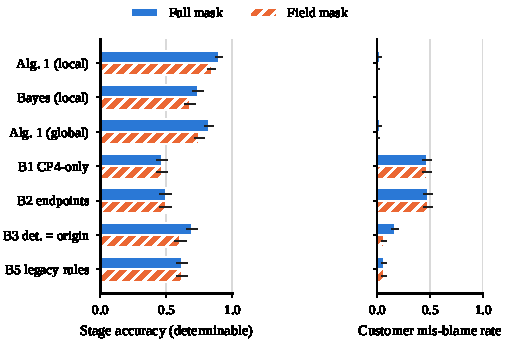
\includegraphics[width=0.76\columnwidth]{fig/fig2_e1.pdf}
\caption{Stage accuracy (determinable journeys) and customer mis-blame under the full and field masks, with 95\% bootstrap intervals; simulated test journeys.}
\label{fig:e1}
\end{figure}

The Bayesian variant trades accuracy for caution. It never blamed the customer wrongly and never accused a legitimate journey (\BayMis\% and \BayFA\%), yet its accuracy was \BayAcc\%. When one trusted modality reports a change and two report none, the likelihood product favours \LEG, so single-modality evidence is outvoted. Algorithm~1 accepts any trusted anomaly and so detects these changes, at the cost of \AlgFA\% false accusations that arise from nuisance effects (Section~\ref{sec:errors}).

\subsection{Global Versus Local Visual Comparison}
\label{sec:visual}
Most of the gap to the preregistered global score (\GloAcc\%) lies in forward-transit damage, where the dent is the only strong signal. Accuracy there was \FwdGlo\% with the global score and \FwdAlg\% with the local score (Table~\ref{tab:cells}). A check on 40 pairs of simulated faces explains the difference. For two photographs of the same untouched face, the median global score is \VisGloPose{} under the nominal pose displacement and \VisGloNoPose{} with identical pose, whereas a clearly visible mark raises it only to \VisGloMark{} even with identical pose. On untouched pairs the local score never exceeded \VisLocIntactMax, while marks of moderate visibility scored at least \VisLocMarkMin. Across simulated pose displacements of 0--24\,px, Algorithm~1 stayed between \SwPoseMinAlg\% and \SwPoseMaxAlg\%.

\begin{table}[t]
\caption{Scenario Cells and Stage Accuracy by Cell (Full Mask)}
\label{tab:cells}
\centering
\footnotesize
\setlength{\tabcolsep}{1.0pt}
\begin{tabular}{@{}lccccccccc@{}}
\toprule
Cell & Truth & $n$ & Test & Det. & Alg.\,1 & Glob. & Bayes & B1 & B3 \\
\midrule
Intact & LEG & 240 & 192 & 188 & 0.899 & 0.920 & 0.989 & 0.835 & 0.649 \\
Flyer replaced, logged & LEG & 96 & 77 & 75 & 0.840 & 0.853 & 1.000 & 0.747 & 0.600 \\
Forward-transit damage & $S_1$ & 112 & 90 & 89 & 0.854 & 0.270 & 0.000 & 0.000 & 0.674 \\
Doorstep substitution & $S_1$ & 112 & 90 & 87 & 0.989 & 0.989 & 0.874 & 0.000 & 0.851 \\
Customer tamper & $S_2$ & 112 & 90 & 82 & 0.927 & 0.915 & 0.598 & 0.780 & 0.805 \\
Reverse-transit tamper & $S_3$ & 96 & 77 & 74 & 0.878 & 0.892 & 0.716 & 0.000 & 0.608 \\
Degraded evidence & DEG & 96 & 77 & 0 & (94.8\%) & -- & -- & -- & -- \\
Ambiguous (glare) & IND & 96 & 77 & 0 & (97.4\%) & -- & -- & -- & -- \\
\midrule
Total &  & 960 & 770 & 595 & 0.899 & 0.820 & 0.738 & 0.466 & 0.692 \\
\bottomrule

\end{tabular}

\vspace{2pt}
\parbox{0.96\columnwidth}{\footnotesize $n$: simulated journeys (8$\times$ the protocol size); Test: test journeys; Det.: those with determinable truth, on which accuracy is computed. Parentheses: Algorithm~1's abstention rate on \DEG{} and \IND{} journeys.}
\end{table}

\subsection{Where the Errors Come From}
\label{sec:errors}
Errors concentrate where nuisance effects occur: Algorithm~1 was correct on \NoNuisAcc\% of determinable test journeys without any and on \NuisAcc\% of those with at least one. Of the \FATotal{} legitimate journeys it accused, \FAMisread{} had a misread identifier and \FAGlare{} had glare that the operator did not report; \FABoth{} had both, and in the other \FANeither{} only the CP3 weight exceeded its bound. A misread seal or serial looks exactly like a replaced one, and glare covering less than the gate's 15\% ceiling passes the gate. By tamper strength, accuracy was \MassBig\% when 15\,g or more was removed, \MassSmall\% for 2--15\,g and \MassZero\% for weight-matched tampering, with cloned seals the hardest case (\Cloned\%).

\subsection{Ablations}
Table~\ref{tab:ablation} removes one component at a time. Without the quality gate, appropriate abstention fell from \AbFullAAR\% to \AbNoQAAR\%, unwarranted blame rose to \AbNoQUBR\% and false accusations to \AbNoQFA\%, because dark, blurred and glare-covered photographs were compared as if sound. Without the visual reconciler, accuracy fell by \AbNoVisDrop{} points, mostly on forward-transit damage (\AbFwdFull\% to \AbFwdNoVis\%). Removing the layered seals lowered accuracy on doorstep substitution from \AbDoorFull\% to \AbDoorNoSeal\%, although false accusations dropped to \AbNoSealFA\% because misread seal identifiers no longer raised alarms. Under the field mask, Algorithm~1 fell to \FAlgAcc\% and its unnecessary-abstention rate rose to \FAlgUAR\%, since a change seen only on the scale is then no longer bracketed; customer mis-blame was \FAlgMis\%.

\begin{figure}[t]
\centering
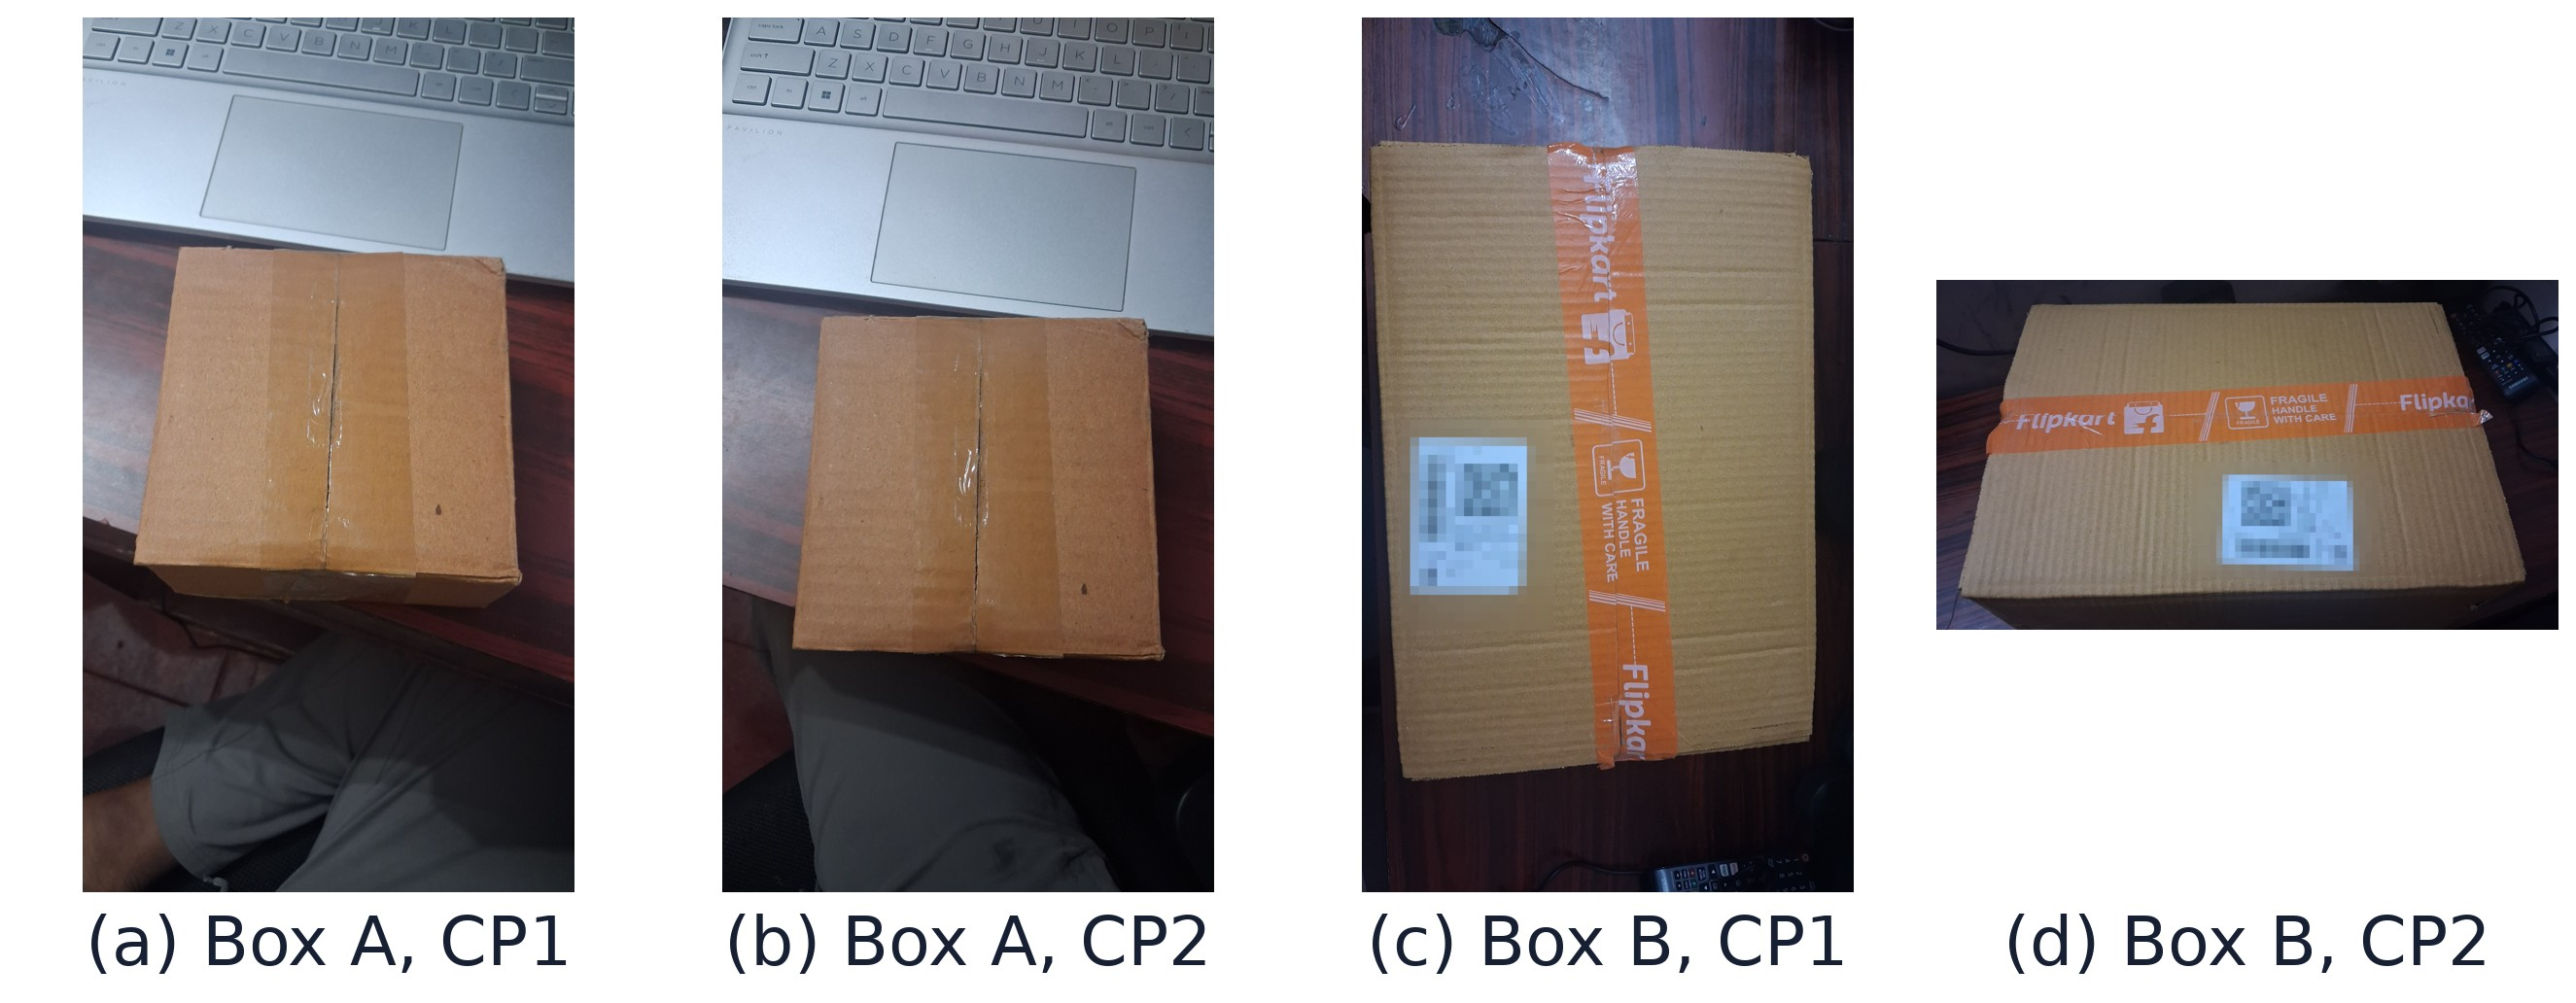
\includegraphics[width=0.70\columnwidth]{fig/fig4_real.jpg}
\caption{First real captures (labels pixelated). Box~A (a, b) was correctly found legitimate; Box~B (c, d) was unchanged by weight and seals, but its differently framed CP2 photograph was read as a change.}
\label{fig:real}
\end{figure}

\begin{table}[t]
\caption{Ablations of Algorithm 1 (Full Mask)}
\label{tab:ablation}
\centering
\footnotesize
\setlength{\tabcolsep}{3pt}
\begin{tabular}{@{}lccccc@{}}
\toprule
Variant & Acc. & AAR & UBR & Mis-blame & False acc. \\
\midrule
Full Algorithm 1 & 0.899 & 0.966 & 0.017 & 0.025 & 0.103 \\
No quality gate & 0.805 & 0.429 & 0.531 & 0.109 & 0.308 \\
No visual & 0.766 & 0.943 & 0.029 & 0.023 & 0.034 \\
No layered seals & 0.901 & 0.949 & 0.017 & 0.026 & 0.057 \\
Fixed 10\,g weight test & 0.899 & 0.966 & 0.017 & 0.022 & 0.095 \\
\bottomrule

\end{tabular}
\end{table}

\subsection{Sensitivity}
Fig.~\ref{fig:sweeps} varies one factor at a time on independent 240-journey benchmarks. Without nuisance effects Algorithm~1 attributed \SwNuisZeroAcc\% of determinable journeys correctly; at four times the nominal rates it fell to \SwNuisFourAcc\% with \SwNuisFourUAR\% unnecessary abstention, while customer mis-blame never exceeded \SwNuisMaxMis\%. Scale noise hurts the fixed-threshold baselines most: at four times the nominal noise, B3 accused \SwSigFourBthreeFA\% of legitimate journeys and B1 wrongly blamed the customer in \SwSigFourBoneMis\% of cases. Algorithm~1, whose weight tolerance grows with the characterised noise, kept \SwSigFourAlgAcc\% accuracy by abstaining more often (\SwSigFourAlgUAR\% UAR).

\begin{figure*}[t]
\centering
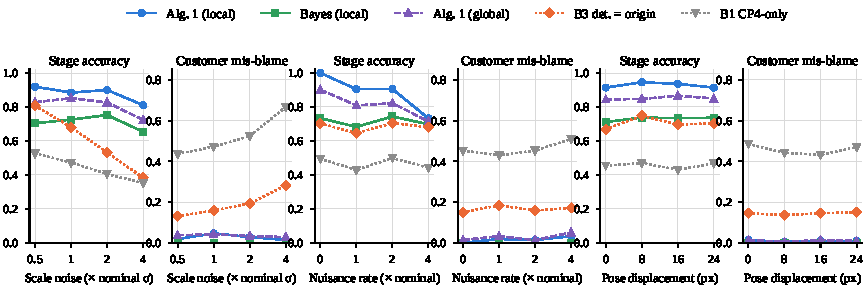
\includegraphics[width=\textwidth]{fig/fig3_sweeps.pdf}
\caption{Sensitivity of stage accuracy and customer mis-blame to scale noise, nuisance rate and camera pose displacement (independent simulated benchmarks of 240 journeys).}
\label{fig:sweeps}
\end{figure*}

\subsection{First Real Captures}
\label{sec:real}
Two real parcels were taken through all four checkpoints with a phone camera and a kitchen scale (Fig.~\ref{fig:real}), as a feasibility check, too few to measure accuracy. Box~A, never opened, had a median weight of 450\,g at every checkpoint against a 2.5\,g limit, its seals were unchanged, and Algorithm~1 returned \LEG. Its CP4 photographs were copies of CP3's, which a reused-photo check now flags. The record of Box~B also shows no change (750\,g throughout, seals unchanged), yet Algorithm~1 attributed a change to $S_1$. CP1 had been photographed upright and CP2 sideways from further away, and on these untouched faces the local score reached 0.72 to 0.75, far above the $\gamma=0.06$ fitted on rendered images. The sharpness floor, set for 640$\times$480 images, also marked several sharp 9-megapixel photographs as blurred. Both thresholds must therefore be refitted on the physical calibration split; the capture application now overlays each face's CP1 photograph so later checkpoints are framed alike.

\section{Discussion and Limitations}\label{sec:disc}
Misread identifiers cause most remaining false accusations, which argues for scanning seals. Apart from the two real captures, every result comes from a simulator that encodes its authors' assumptions; the \AlgAcc\% accuracy and the other figures in Section~\ref{sec:results} describe that model, not field performance. Rendered faces are simpler than real cardboard, tamper marks are drawn instead of cut, and the nuisance probabilities are plausible but unmeasured. The design rules limit direct bias without showing that real errors occur at these frequencies, and the rendered texture and exposure were adjusted until untouched photographs passed the quality floors. The local score and the reference-trust rule were developed on a separate benchmark with a different seed.

A preregistered~\cite{nosek} physical study (protocol v2.6) will stage 120 journeys in the cells of Table~\ref{tab:cells}, split 24/96, with truth from a filmed staging log, a 10-journey pilot and scale characterisation. A datasheet~\cite{gebru} will document its dataset.

\section{Conclusion}
Requiring trusted evidence on both sides of a stage, and abstaining otherwise, kept customer mis-blame at \AlgMis\% in simulation, against \BoneMis\% for inspection at the return hub alone. It also showed that abstention depends on the quality gate (Table~\ref{tab:ablation}) and that global similarity missed small tamper marks under realistic camera pose. The first real captures add that visual thresholds must be refitted on photographs taken with a framing guide. The physical study will test all three.

\section*{Acknowledgment}
We thank the Department of AI and Data Science, Saveetha Engineering College. Code and protocol (MIT licence): \url{github.com/dharshan7200/TriNetraAI}.

\emph{Use of generative AI.} Claude (Anthropic) was used to write most of the code, run the simulation study, produce Figs.~\ref{fig:pipeline}, \ref{fig:e1} and~\ref{fig:sweeps}, assemble Fig.~\ref{fig:real} from the authors' photographs, and draft and edit the text of all sections. The authors directed the work, captured the two real parcels, checked the manuscript and take full responsibility for its content.

\balance
\bibliographystyle{IEEEtran}
\bibliography{refs}

\end{document}
